\documentclass[twoside]{article}
\usepackage[a4paper]{geometry}
\geometry{verbose,tmargin=2.5cm,bmargin=2cm,lmargin=2cm,rmargin=2cm}
\usepackage{fancyhdr}
\pagestyle{fancy}

% nastavení pisma a~češtiny
\usepackage{lmodern}
\usepackage[T1]{fontenc}
\usepackage[utf8]{inputenc}
\usepackage[czech]{babel}

% odkazy
\usepackage{url}

\usepackage{float}
% vícesloupcové tabulky
\usepackage{multirow}
\usepackage{listings}
\usepackage{xcolor}
\usepackage{amssymb}
\usepackage{gensymb}
\usepackage{bbold}
\usepackage{amsmath}
\usepackage{siunitx}
\usepackage{mathtools}
\usepackage{commath}

% vnořené popisky obrázků
\usepackage{subcaption}

% automatická konverze EPS 
\usepackage{graphicx} 
\usepackage{epstopdf}
\epstopdfsetup{update}

\graphicspath{{./images}}

% odkazy a~záložky
\usepackage[unicode=true, bookmarks=true,bookmarksnumbered=true,
bookmarksopen=false, breaklinks=false,pdfborder={0 0 0},
pdfpagemode=UseNone,backref=false,colorlinks=true] {hyperref}


% Poznámky při překladu
\usepackage{xkeyval}	% Inline todonotes
\usepackage[textsize = footnotesize]{todonotes}
\presetkeys{todonotes}{inline}{}

%https://tex.stackexchange.com/questions/2783/bold-calligraphic-typeface
\DeclareMathAlphabet\mathbfcal{OMS}{cmsy}{b}{n}

% enumerate zacina s pismenem
\renewcommand{\theenumi}{\alph{enumi}}

% smaz aktualni page layout
\fancyhf{}
% zahlavi
\usepackage{titling}
\fancyhf[HC]{\thetitle}
\fancyhf[HLE,HRO]{\theauthor}
\fancyhf[HRE,HLO]{\today}
 %zapati
\fancyhf[FLE,FRO]{\thepage}

% údaje o autorovi
\title{OTE Domácí úkol 6b - Horní propust}
\author{Vojtěch Michal}
\date{\today}

%customize code listing
\definecolor{codegreen}{rgb}{0,0.6,0}
\definecolor{codegray}{rgb}{0.5,0.5,0.5}
\definecolor{codepurple}{rgb}{0.58,0,0.82}
\definecolor{backcolour}{rgb}{0.95,0.95,0.92}

\lstdefinestyle{mystyle}{
    backgroundcolor=\color{backcolour},   
    commentstyle=\color{codegreen},
    keywordstyle=\color{magenta},
    numberstyle=\tiny\color{codegray},
    stringstyle=\color{codepurple},
    basicstyle=\ttfamily\footnotesize,
    breakatwhitespace=false,         
    breaklines=true,                 
    captionpos=b,                    
    keepspaces=true,                 
    numbers=left,                    
    numbersep=5pt,                  
    showspaces=false,                
    showstringspaces=false,
    showtabs=false,                  
    tabsize=2
}

\lstset{style=mystyle}

\begin{document}

\maketitle

V simulacích pro tuto úlohu bylo použito standardní nastavení parametrů operačního zesilovače,
které však s ohledem na charakter úlohy nemá významný vliv. Tranzitní kmitočet použitého OZ je $f_T = 1 \si{\mega\hertz}$.

Použitím hodnot $C = 10 \si{\nano\farad}$ a $R = 10 \si{\kilo\ohm}$
vychází mezní frekvence horní propusti
\begin{equation}
    f_m = \frac{1}{2 \pi R C} = 1592 \si{\hertz}.
\end{equation}

V závislosti na použitém typu aproximace je nastavováno zesílení 
\begin{equation}
    G_\infty = \frac{R_3 + R_4}{R_4} \in \langle 1; 3 \rangle.
\end{equation}

\section{Frekvenční charakteristika}

S pomocí zapojení na schématu \ref{fig:schema_bode} a funkce \textit{AC sweep} byly
získány frekvenční charakteristiky všech aproximací horní propusti,
které jsou vykresleny na obrázkách \ref{fig:bode_kriticke}, \ref{fig:bode_bessel}, \ref{fig:bode_butter} a \ref{fig:bode_cebysev}.
Srovnání vypočtených a změřených veličin je v tabulce \ref{tab:filtry}.
Teoretické zlomové frekvence byly vypočítány nalezeném takového přirozeného $f$, které splňuje
\begin{equation}
    \left| \frac{-(\frac{f}{f_0})^2}{1+i\frac{f}{f_0} (3-G_{\infty}) - (\frac{f}{f_0})^2} \right| \approx \frac{\sqrt{2}}{2}.
\end{equation}

\begin{table}
    \centering
    \begin{tabular}{c|c|c|c}
        aproximace & zesílení $G_{\infty}$ & vypočtená $f_m$ & změřená $f_m$ \\ \hline
        kritické tlumení & 1 (-0,059 dB) & 2478 \si{\hertz} & 2419 \si{\hertz} \\
        Bessel & 1,268 (1,97 dB) & 2028 \si{\hertz} & 1983 \si{\hertz} \\
        Butterworth & 1,586 (3,86 dB)  & 1595 \si{\hertz} & 1555 \si{\hertz} \\
        Čebyšev & 2,234 (6,71 dB) & 1146 \si{\hertz}& 1126 \si{\hertz}
    \end{tabular}
    \label{tab:filtry}
    \caption{Vlastnosti různých aproximací filtru}
\end{table}

\begin{figure}[h!]
    \centering
    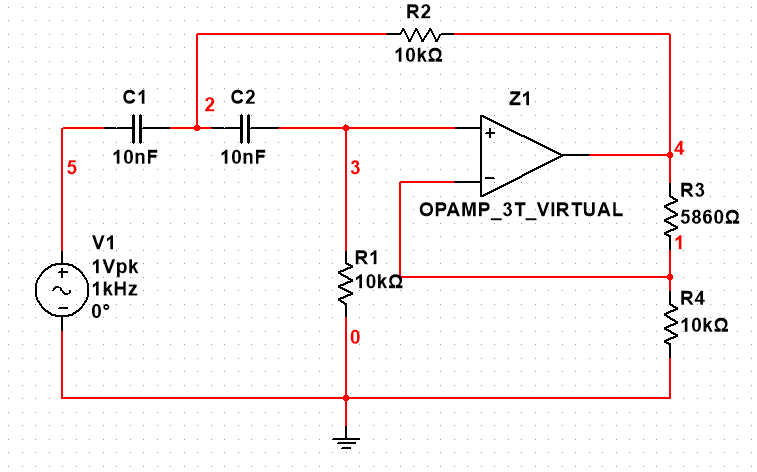
\includegraphics[width=0.55\linewidth]{bode_schema.png}
    \caption{Horní propust dle Butterworthovy aproximace}
    \label{fig:schema_bode}
\end{figure}

\newpage
\begin{figure}[h!]
    \centering
    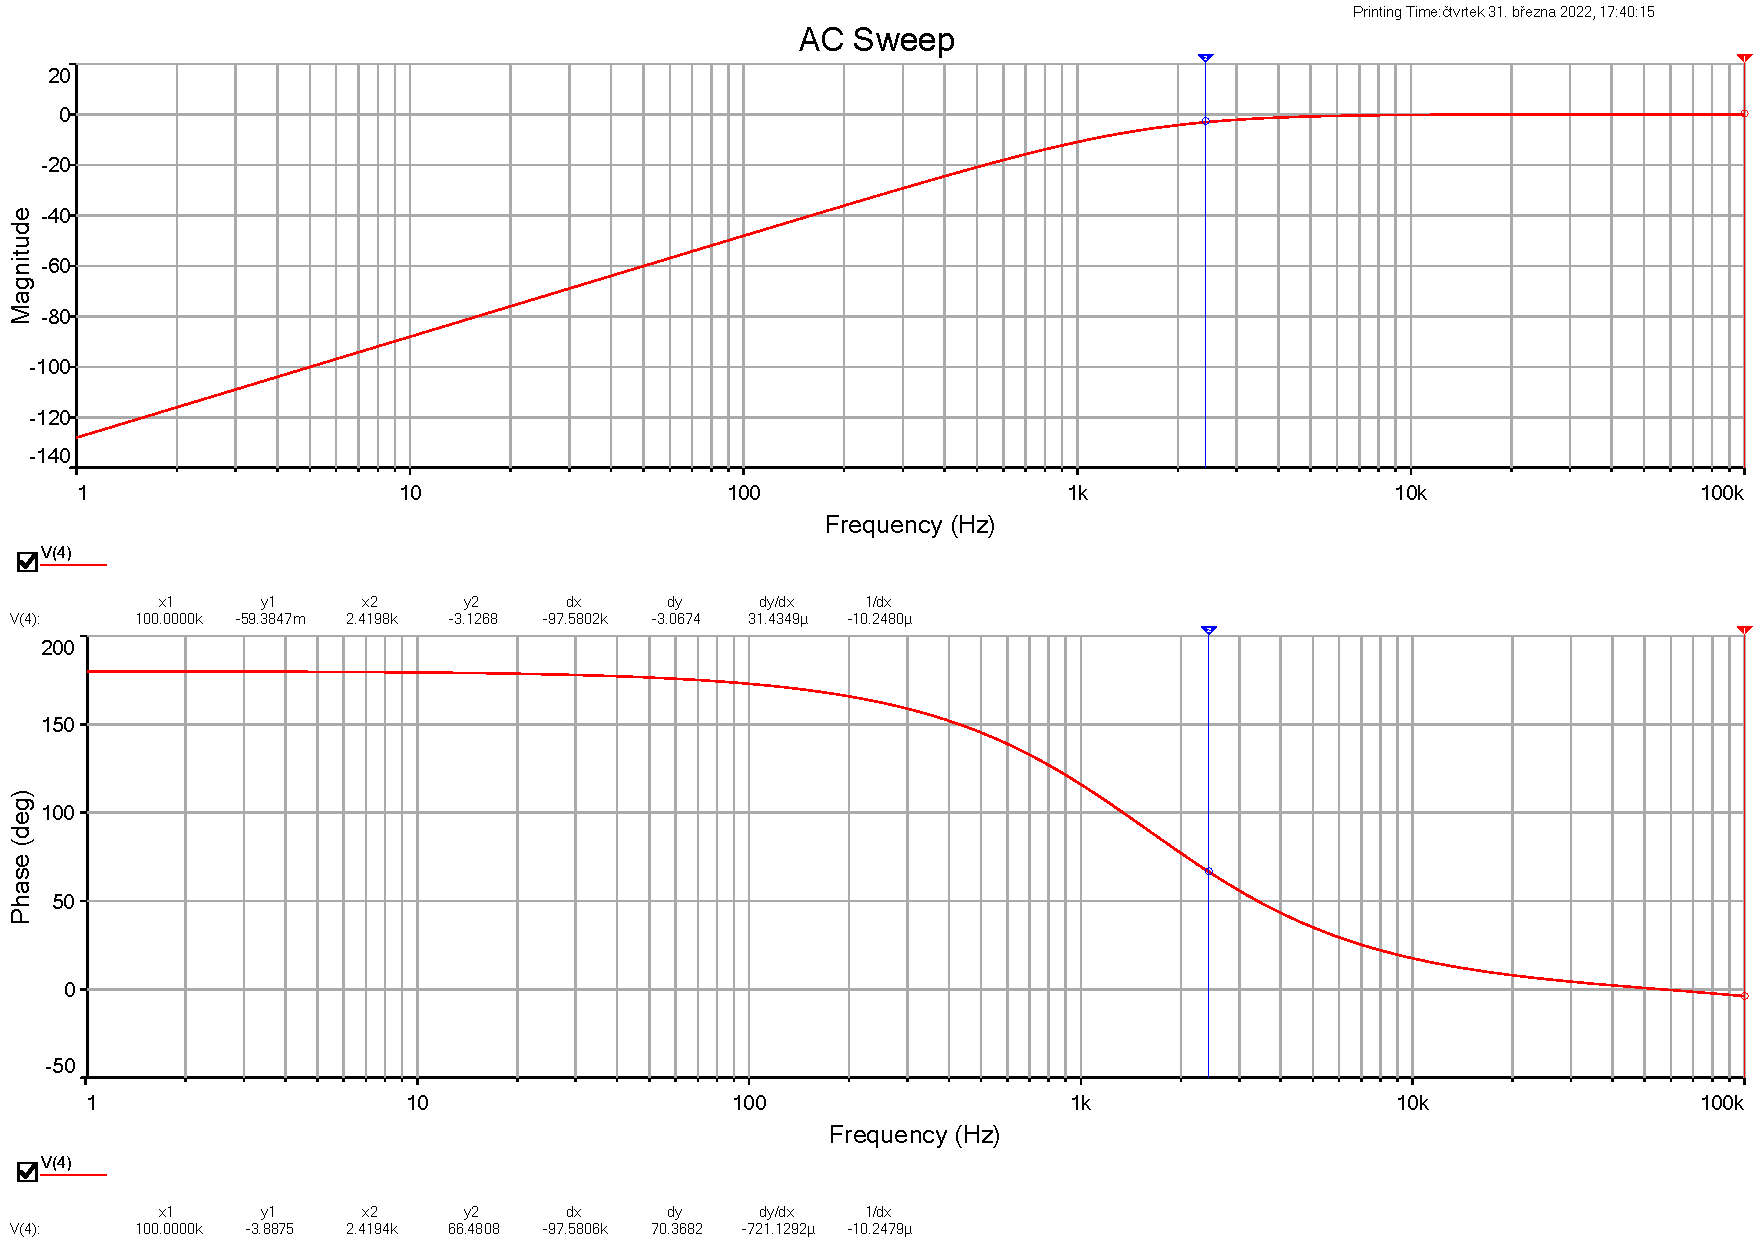
\includegraphics[width=0.92\linewidth]{bode_kriticke.pdf}
    \caption{Frekvenční charakteristika pro kritické tlumení ($G_{\infty} = 1$)}
    \label{fig:bode_kriticke}
\end{figure}

\begin{figure}[h!]
    \centering
    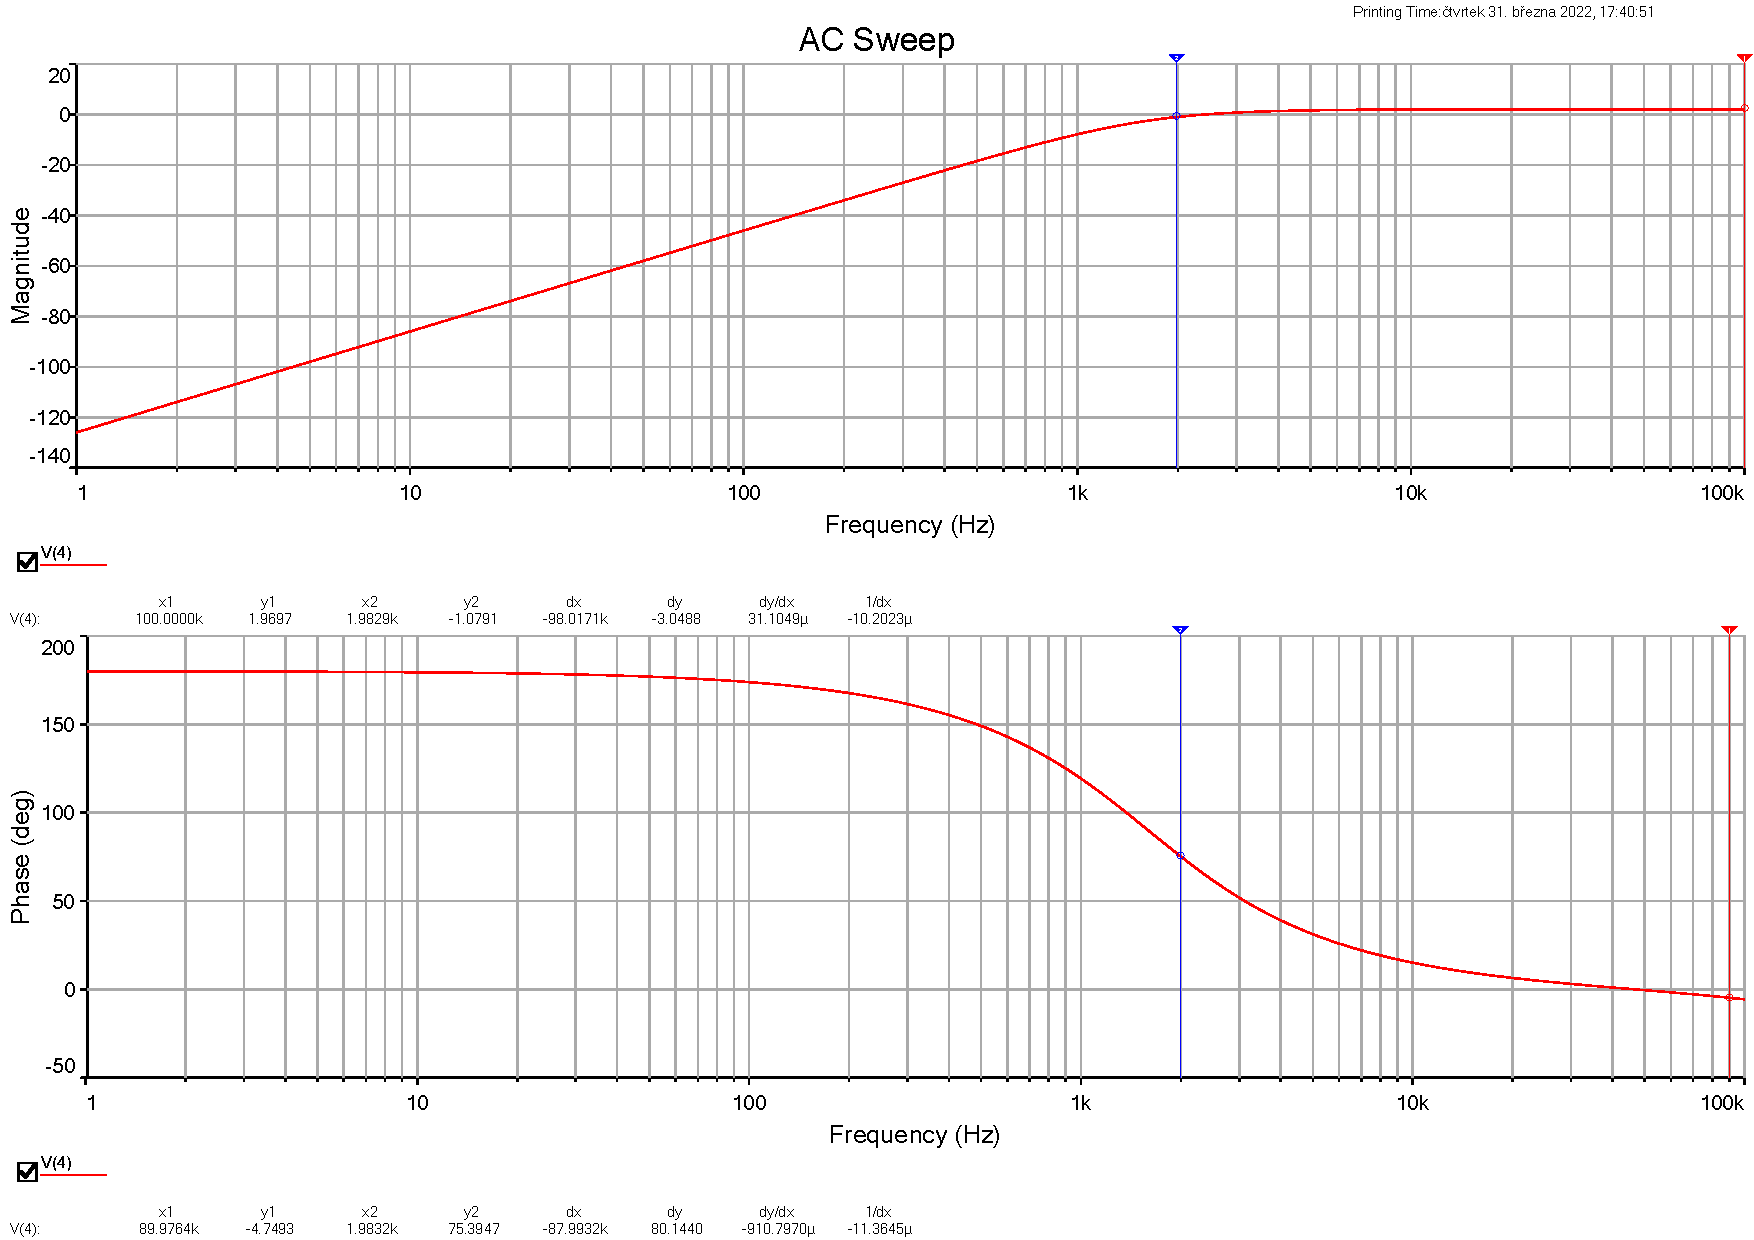
\includegraphics[width=0.92\linewidth]{bode_bessel.pdf}
    \caption{Frekvenční charakteristika pro Besselovu aproximaci ($G_{\infty} = 1,268$)}
    \label{fig:bode_bessel}
\end{figure}

\begin{figure}[h!]
    \centering
    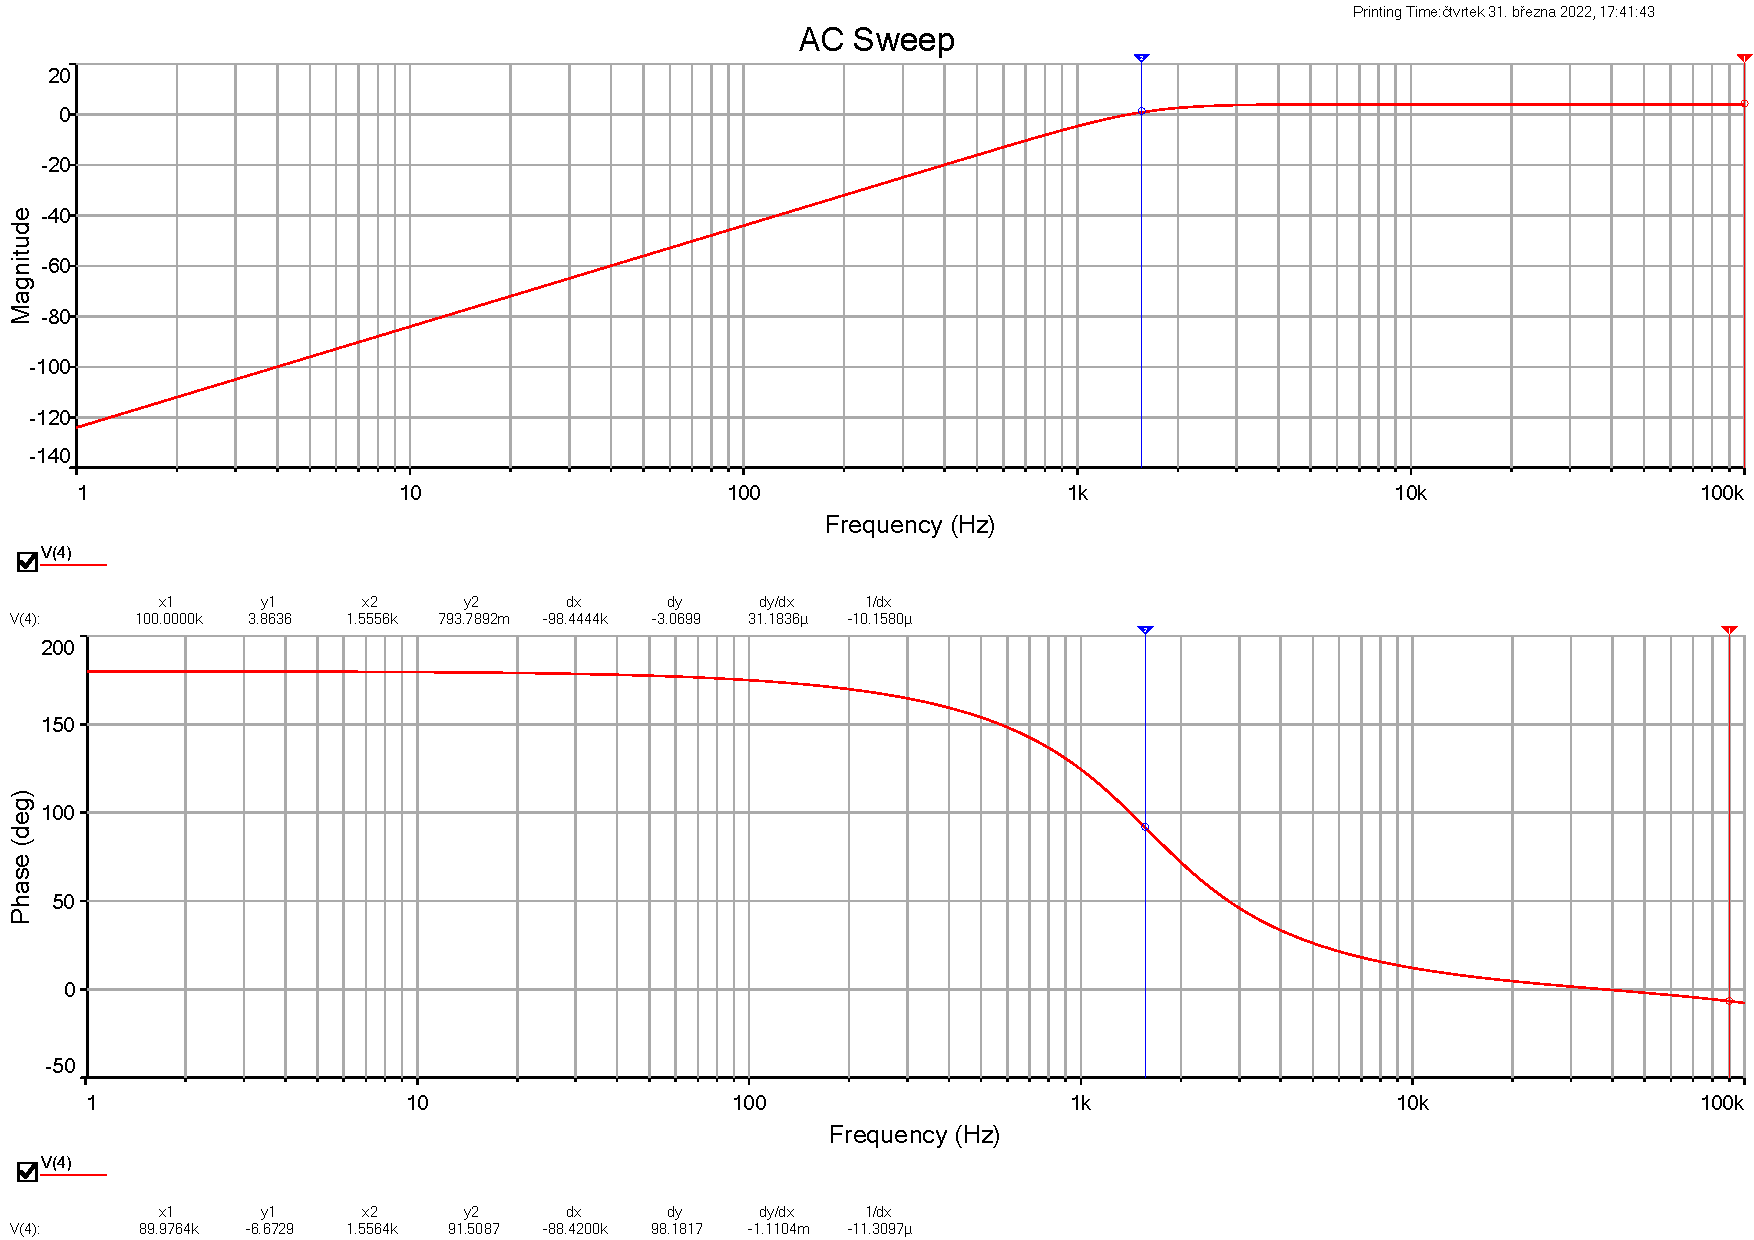
\includegraphics[width=0.92\linewidth]{bode_butter.pdf}
    \caption{Frekvenční charakteristika pro Butterworthovu aproximaci ($G_{\infty} = 1,586$)}
    \label{fig:bode_butter}
\end{figure}

\begin{figure}[h!]
    \centering
    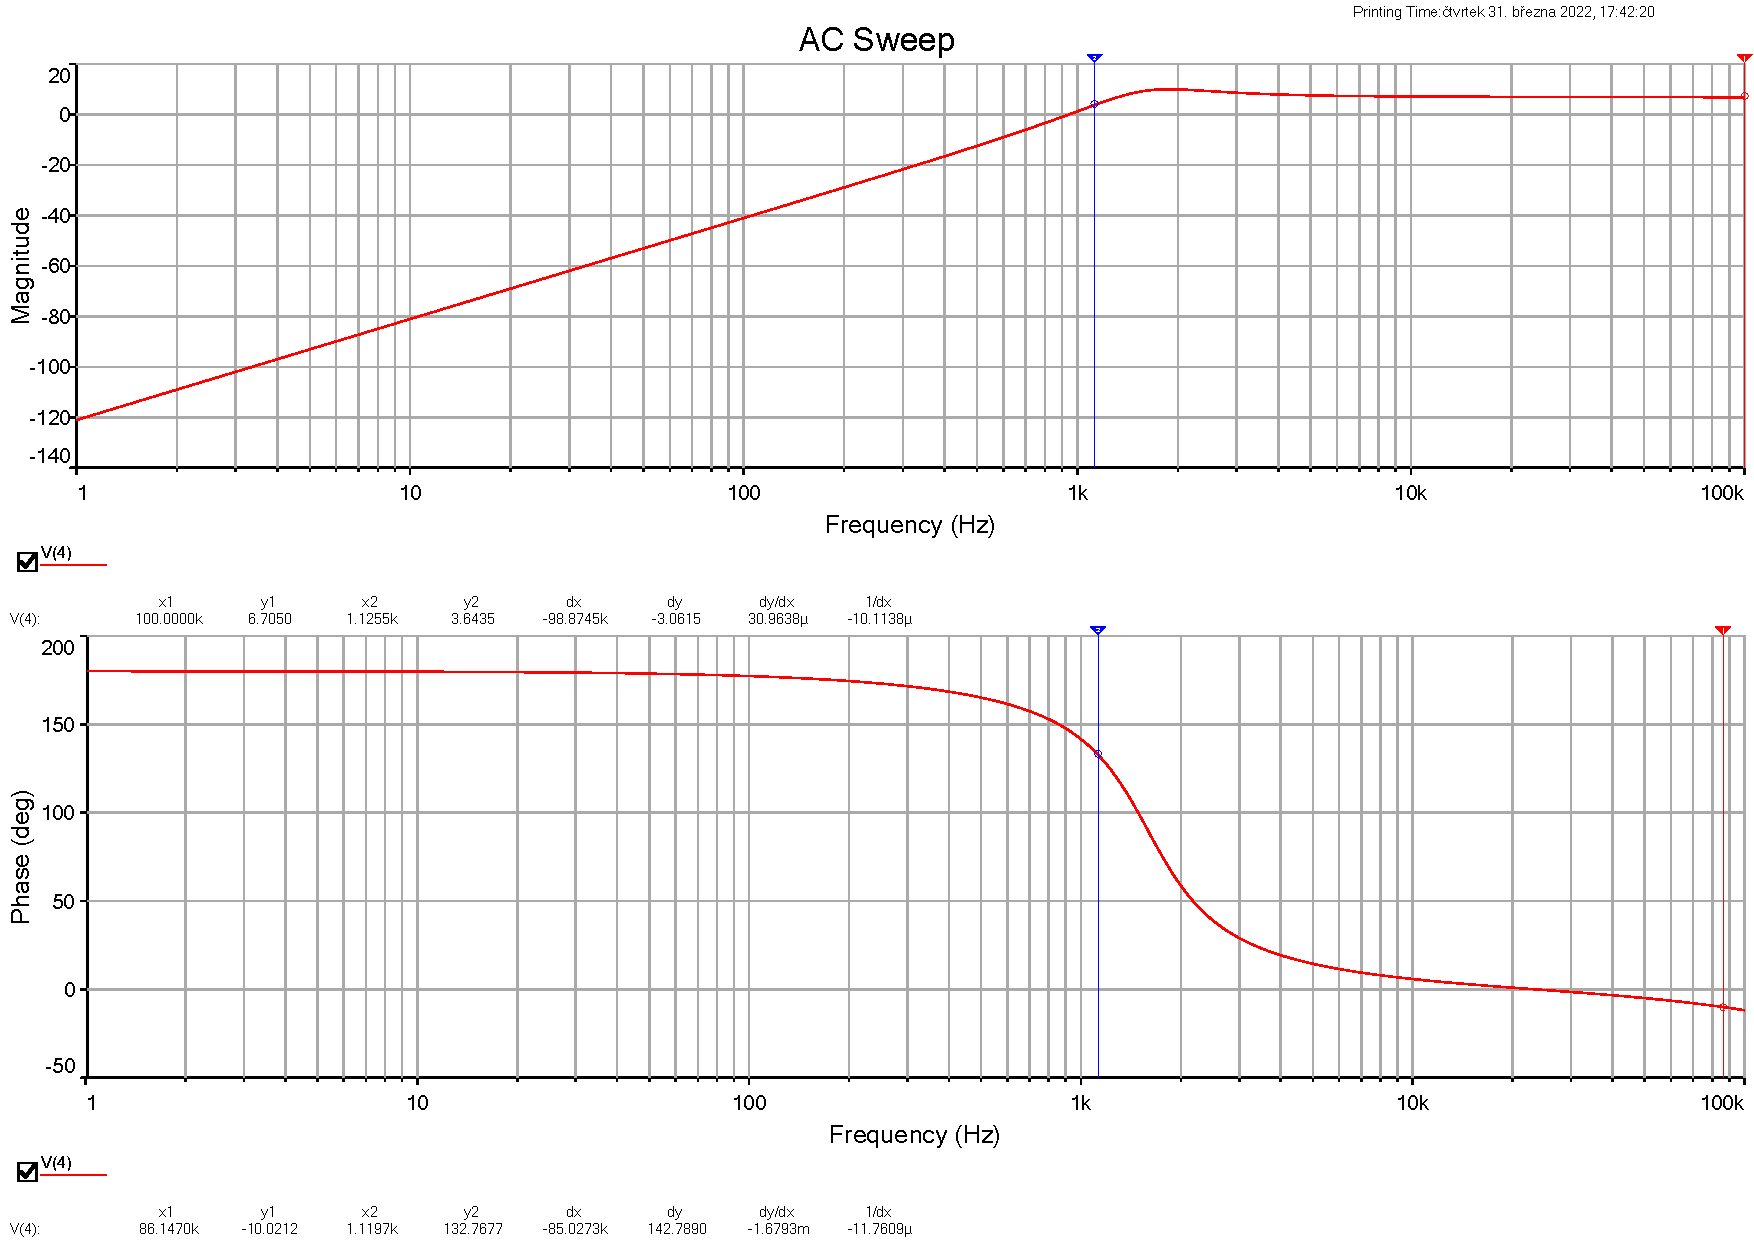
\includegraphics[width=0.92\linewidth]{bode_cebysev.pdf}
    \caption{Frekvenční charakteristika pro Čebyševovu aproximaci ($G_{\infty} = 2,234$)}
    \label{fig:bode_cebysev}
\end{figure}

\newpage
\section{Přechodová charakteristika}

\begin{figure}[h!]
    \centering
    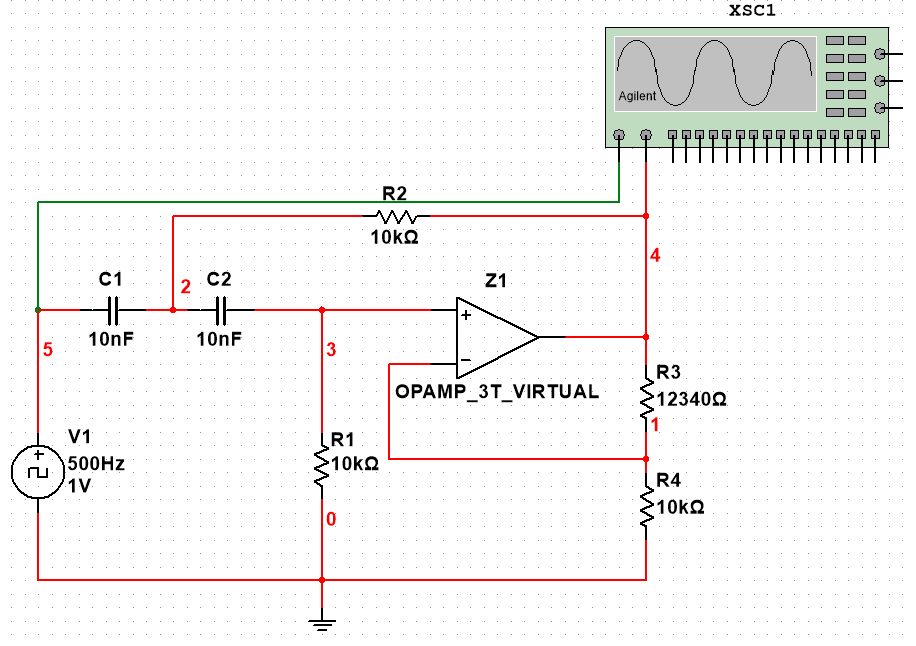
\includegraphics[width=0.8\linewidth]{step_schema.png}
    \caption{Schéma pro určení přechodové charakteristiky filtru}
    \label{fig:schema_step}
\end{figure}

Na zapojení na schématu \ref{fig:schema_step} bylo změřeno několik přechodových charakteristik
vykreslených na obrázkách \ref{fig:step}. Na vstup filtru byl připojen budicí signál 
obdélníkového tvaru s amplitudou 1 V a frekvencí 300 Hz. Rozlišení na svislé ose je 
rovněž stejné (1 V na dílek) s výjimkou \ref{fig:step_15k} a \ref{fig:step_19k}, kde musel být krok na svislé ose upraven,
aby byl vidět plný rozkmit výstupu filtru.

Charakteristiky \ref{fig:step_kriticke} až \ref{fig:step_cebysev} vypadají podle očekávání -- 
s rostoucím zesílením $G_{\infty}$ roste i míra oscilací po první špičce a systém se pomalu stává nestabilní. Na charakteristice 
\ref{fig:step_15k} již jsou pozorovatelné kmity, které se ani neustálí během celé půlperiody budicího signálu. Poslední průběh s $G_{\infty} = 2,995$ ukazuje,
jak filtr kmitá skoro bez ohledu na hrany budicího signálu a tlumení je naprosto minimální.

\begin{figure}[h!]
    \centering
    \begin{subfigure}{0.48\textwidth}
        \centering
        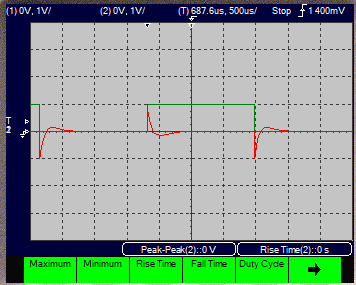
\includegraphics[width=1\linewidth]{step_kriticke.png}
        \caption{Kritické tlumení $G_{\infty} = 1$}
        \label{fig:step_kriticke}
    \end{subfigure}
    \begin{subfigure}{0.48\textwidth}
        \centering
        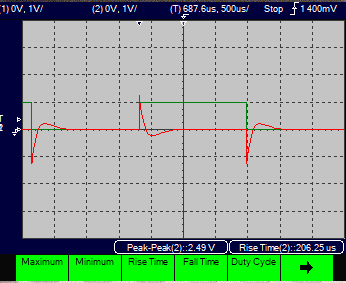
\includegraphics[width=1\linewidth]{step_bessel.png}
        \caption{Besselova aproximace $G_{\infty} = 1,268$}
        \label{fig:step_bessel}
    \end{subfigure}

    \begin{subfigure}{0.48\textwidth}
        \centering
x        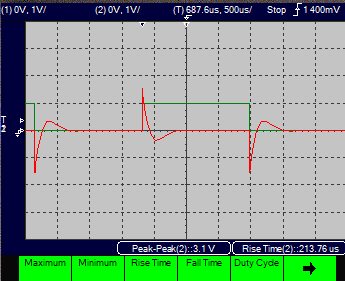
\includegraphics[width=1\linewidth]{step_butter.png}
        \caption{Butterworhova aproximace $G_{\infty} = 1,586$}
        \label{fig:step_butter}
    \end{subfigure}
    \begin{subfigure}{0.48\textwidth}
        \centering
        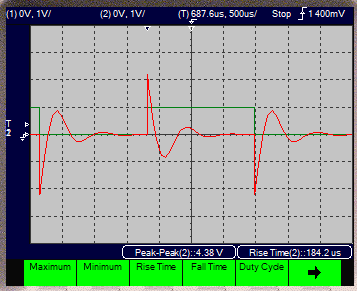
\includegraphics[width=1\linewidth]{step_cebysev.png}
        \caption{Čebyševova aproximace $G_{\infty} = 2,234$}
        \label{fig:step_cebysev}
    \end{subfigure}

    \begin{subfigure}{0.48\textwidth}
        \centering
        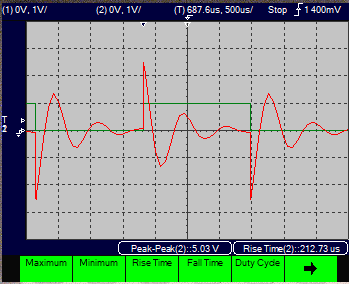
\includegraphics[width=1\linewidth]{step_15k.png}
        \caption{Zesílení $G_{\infty} = 2,5$}
        \label{fig:step_15k}
    \end{subfigure}
    \begin{subfigure}{0.48\textwidth}
        \centering
        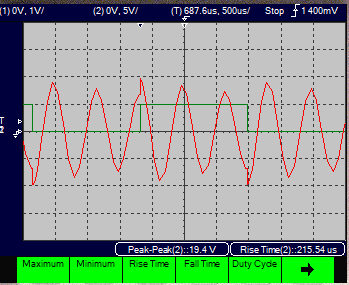
\includegraphics[width=1\linewidth]{step_19k5.png}
        \caption{Zesílení $G_{\infty} = 2,95$}
        \label{fig:step_19k}
    \end{subfigure}

    \caption{Přechodové charakteristiky filtru pro různá zesílení $G_{\infty}$}
    \label{fig:step}
\end{figure}

\end{document}

